\chapter{Procedure and Data}

\section{Setup}
\begin{figure}
	\centering
	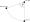
\includegraphics[width=.4\textwidth]{./img/setup.pdf}
	\captiond{The setup}{used in this experiment}
	\label{fig:setup}
\end{figure}
The setup consists of a scintillation detector, consisting of a NaI-scintillator crystal and a sensitive photomultiplier tube (PMT), a small pedestal, the targets are mounted on and the gamma sources themselves.
Sodium iodide is an inorganic scintillator crystal, giving the advantage of most of the gamma rays being observed through the photoelectric effect.

The angle enclosed by the lines of sight detector-target, target-source can be varied to observe photons of different scattering angle $\Theta$.
Measurements are carried out for angles between \num{25} and \SI{105}{\degree}, with a duration of \SI{300}{\second} both with and without the target.

To determine the dependency of the differential cross-section on the atomic number $Z$, four different target materials (Al, Cu, Fe, Pb) are available.

For the dimensions of all materials used in the experiment, see the lab manual (blue book).

\section{Calibration}
\begin{figure}
	\centering
	\includegraphics[scale=0.8]{./data/plots/calibration.pdf}
	\captiond{Energy calibration}{. The vertical black lines show the approximation for the peak channel, which is used as initial parameter for each gaussian fit. Successful fits are also shown in black. The initial approximation is based on the peaks of Co-57 and Co-60. Cs-137 matches this approximation very well, while both peaks of Na-22 are significantly shifted to the right. For this reason, Na-22 is not used in the final calibration. }
	\label{fig:calib}
\end{figure}
Every detector channel corresponds to a specific energy.
If an exact linear relationship between channel number and energy is assumed, all that is needed for energy calibration is a gamma source that emits radiation peaks of a known energy.
In this experiment, more than one standard source is used for energy calibration to account for non-linear behavior of the detector.
Using
\begin{equation*}
	E = a\cdot C + b,
\end{equation*}
where $E$ and $C$ denote the channel energy and number respectively, a best fit is applied to determine $a$ and $b$.
Used sources are Co-57, Co-60 and Cs-137.

In \autoref{fig:calib}, known peak energy values are assigned to their corresponding peaks.
Using these values, fit coefficients of
\begin{align*}
	a &= \SI{3.605(22)}{\kilo\eV\per\ch} \\
	b &= \SI{20.23(222)}{\kilo\eV}
\end{align*}
are determined.

\section{Corrections}
For every measurement carried out in this experiment, counts are corrected according to the formula
\begin{equation*}
	N_\text{corr.} = N_\text{obs.} - N_\text{base},
\end{equation*}
where $N_\text{obs.}$ is the observed count and $N_\text{base}$ denotes the baseline noise count for the measurement.

The value for $N_\text{base}$ is acquired by conducting a measurement while the target is not present.

\section{Errors}
The number of decay events from a radioactive source obeys a Poisson distribution.
For this distribution, a good estimate of its standard deviation is the square root of the count
\begin{equation*}
	\sigma = \sqrt{N_\text{obs.} + N_\text{base}}.
\end{equation*}
This statistic error is assumed for all count rates in this experiment.

\section{Differential Cross-Section}\label{sec:diff_cross_res}
\begin{figure}
	\centering
	\includegraphics[scale=0.8]{./data/plots/diff-cross-sec.pdf}
	\caption{Differential cross-section over scatter angle}
	\label{fig:diff_cross}
\end{figure}

The count of every channel is multiplied with the inverse quantum efficiency of the detector (as provided in the experiment manual) and summed up to obtain the total number of scattered photons.
\autoref{fig:diff_cross} shows the determined differential cross-section $\frac{\d\sigma}{\d\Omega}$ over the scatter angle $\theta$.
For comparison, the theoretical model established in \autoref{eq:kleinnishina} is plotted as well.
It is easy to see that the data is not in accordance with the model.
However, the general shape of the data remotely resembles the model and suggests that an unknown systemic error has not been taken into account.
Next-to-leading-order (NLO) corrections to the process cannot compensate this error, since they should be of order $\mathcal{O}(\alpha^2)$.

\section{Electron Mass Estimation by Compton Energy Shift}
\begin{figure}
	\centering
	\includegraphics[scale=0.8]{./data/plots/energy-shift.pdf}
	\captiond{Inverse energy of scattered photons $E^{'-1}$ over function $\left(1-\cos\theta\right)$}{of scattering angle $\Theta$. The energy is the center of a gaussian fit, similar to \autoref{fig:calib}. Points are not marked with markers, as not to hide the associated error bars. The expected linear dependence is observed.}
	\label{fig:energy_shift}
\end{figure}

\autoref{eq:energy_shift} offers a way of estimating the electron mass by measuring the scattered Compton photon's energy for various angles.
Rearranging the equation yields
\begin{equation*}
	\frac{1}{E'_\gamma} = a\cdot\left(1-\cos\theta\right) + b,
\end{equation*}
where according to \autoref{eq:energy_shift} $a=1/m_e$ and $b=\frac{1}{E_\gamma}$.
Note that in these equations, $c$ is set to 1.

Plotting $E_\gamma^{'-1}$ against $1-\cos\theta$ and applying a linear fit yields fit coefficients
\begin{align*}
	a &= \SI{2.151(28)e-6}{\per\eV} \\
	b &= \SI{1.453(21)e-6}{\per\eV},
\end{align*}
which can be used to estimate the electron mass as
\begin{equation*}
	m_e = a^{-1} = \SI{464.81(614)}{\keV}.
\end{equation*}
% PDG: 0.510 998 9461(31) MeV (http://pdg.lbl.gov/)
The measured value deviates from the standard literature value \cite{pdg} ($\approx\SI{511}{\keV}$) by $\approx 9\%$.

It remains unclear as to why our results exhibit such high deviation.
As discussed earlier in \autoref{sec:diff_cross_res}, one possible explanation could be an unnoticed systemic error in the experiment.

\section{Z-Dependence of Compton Scattering} %as in https://journals.aps.org/pr/abstract/10.1103/PhysRev.99.59
Compton scattering mainly occurs at the electrons inside the target, not the nuclei, as the differential cross-section has a $1/m$ dependency on the mass of the charged particle.
This implies that the total rate of scattered photons should be proportional to the total number of electrons in a target, so the value of
\begin{equation}\label{eq_const-stuff}
	\frac{N_\text{corr} A}{\rho Z}
\end{equation}
should remain constant.

To verify this, samples of four metals with similar dimensions are used as targets and measurements similar to \autoref{sec:diff_cross_res} are carried out.
\autoref{tab:z-dep} shows the atomic properties of the samples' elements, the corrected number of photons scattered in \SI{300}{\second} and the value of \autoref{eq_const-stuff}.
The relation seemingly holds for all tested elements but lead.
This is possibly due to the high binding energy of some of lead's inner electrons, reaching as high as \SI{88}{\kilo\eV}\footnote{\url{http://xdb.lbl.gov/Section1/Table_1-1.pdf}}.
Due to the low number of electrons in these tightly bound states, this alone cannot account for the high deviation of $\approx \SI{40}{\percent}$.

\begin{table}
	\centering
	\caption{Scattering rates for identical samples of different metals}
	\label{tab:z-dep}
	\begin{tabular}{cS[table-format=2.0]S[table-format=3.1]S[table-format=2.2]S[table-format=5.0]S[table-format=5.0]}
		\toprule
		{Element}&
		{$Z$}&
		{$A$ (\si{\gram\per\mole})}&
		{$\rho$ (\si{\gram\per\cubic\centi\meter})}&
		{$N_\text{corr}$}&
		{$\frac{N_\text{corr} A}{\rho Z}$ (\si{\mole\centi\meter\cubed})}\\
		\midrule
		Al&	13&	27.0&	2.7&	29378&	22583\\
		Fe&	26&	55.8&	7.87&	84190&	22965\\
		Cu&	29&	63.5&	8.96&	87872&	21490\\
		Pb&	82&	207.2&	11.34&	60648&	13514\\
		\bottomrule
	\end{tabular}
\end{table}
